\section{Depletion voltage}
\label{sec:DepletionVoltage}

The SNR and the parameter $\sigma$ correspond to the most probable value (MPV) and the width of the Landau distribution, as returned by the fit. 

The SNR as a function of the applied bias voltage is shown in Fig. \ref{fig:DepletionVoltageM} for the mini sensors and in Fig. \ref{fig:DepletionVoltageF} for the half size sensor.
The corresponding plots for the parameter $\sigma$ are shown instead in Figs. \ref{fig:DepletionVoltage2M} and \ref{fig:DepletionVoltage2F}.

% Changes as a function of the radiation dose?
% Changes between fan-in and fan-up?
% Changes between back-side and top-side biasing?

\begin{figure}[]
\centering
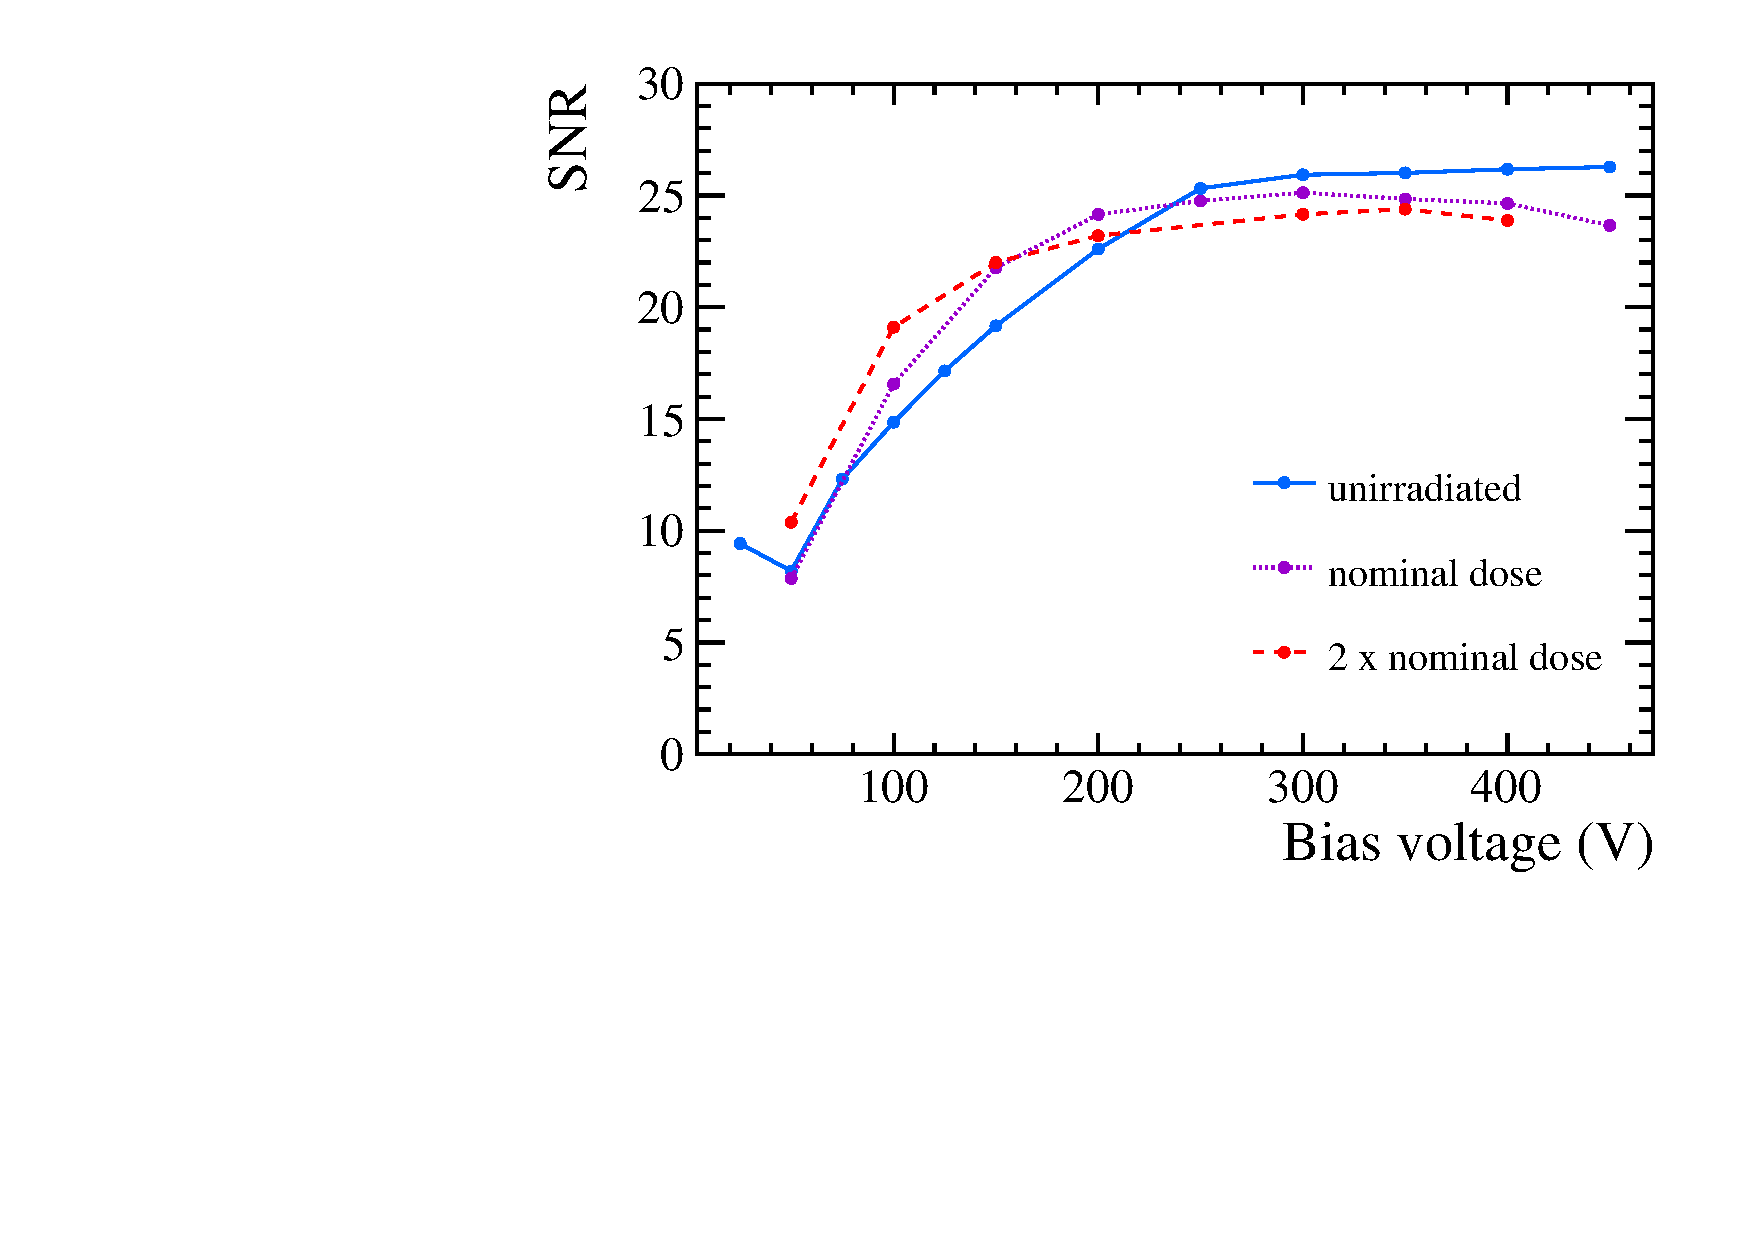
\includegraphics[width=0.47\textwidth]{figs/CombineSNRvsBias/cSNRvsBias_FanIn_Back.pdf}
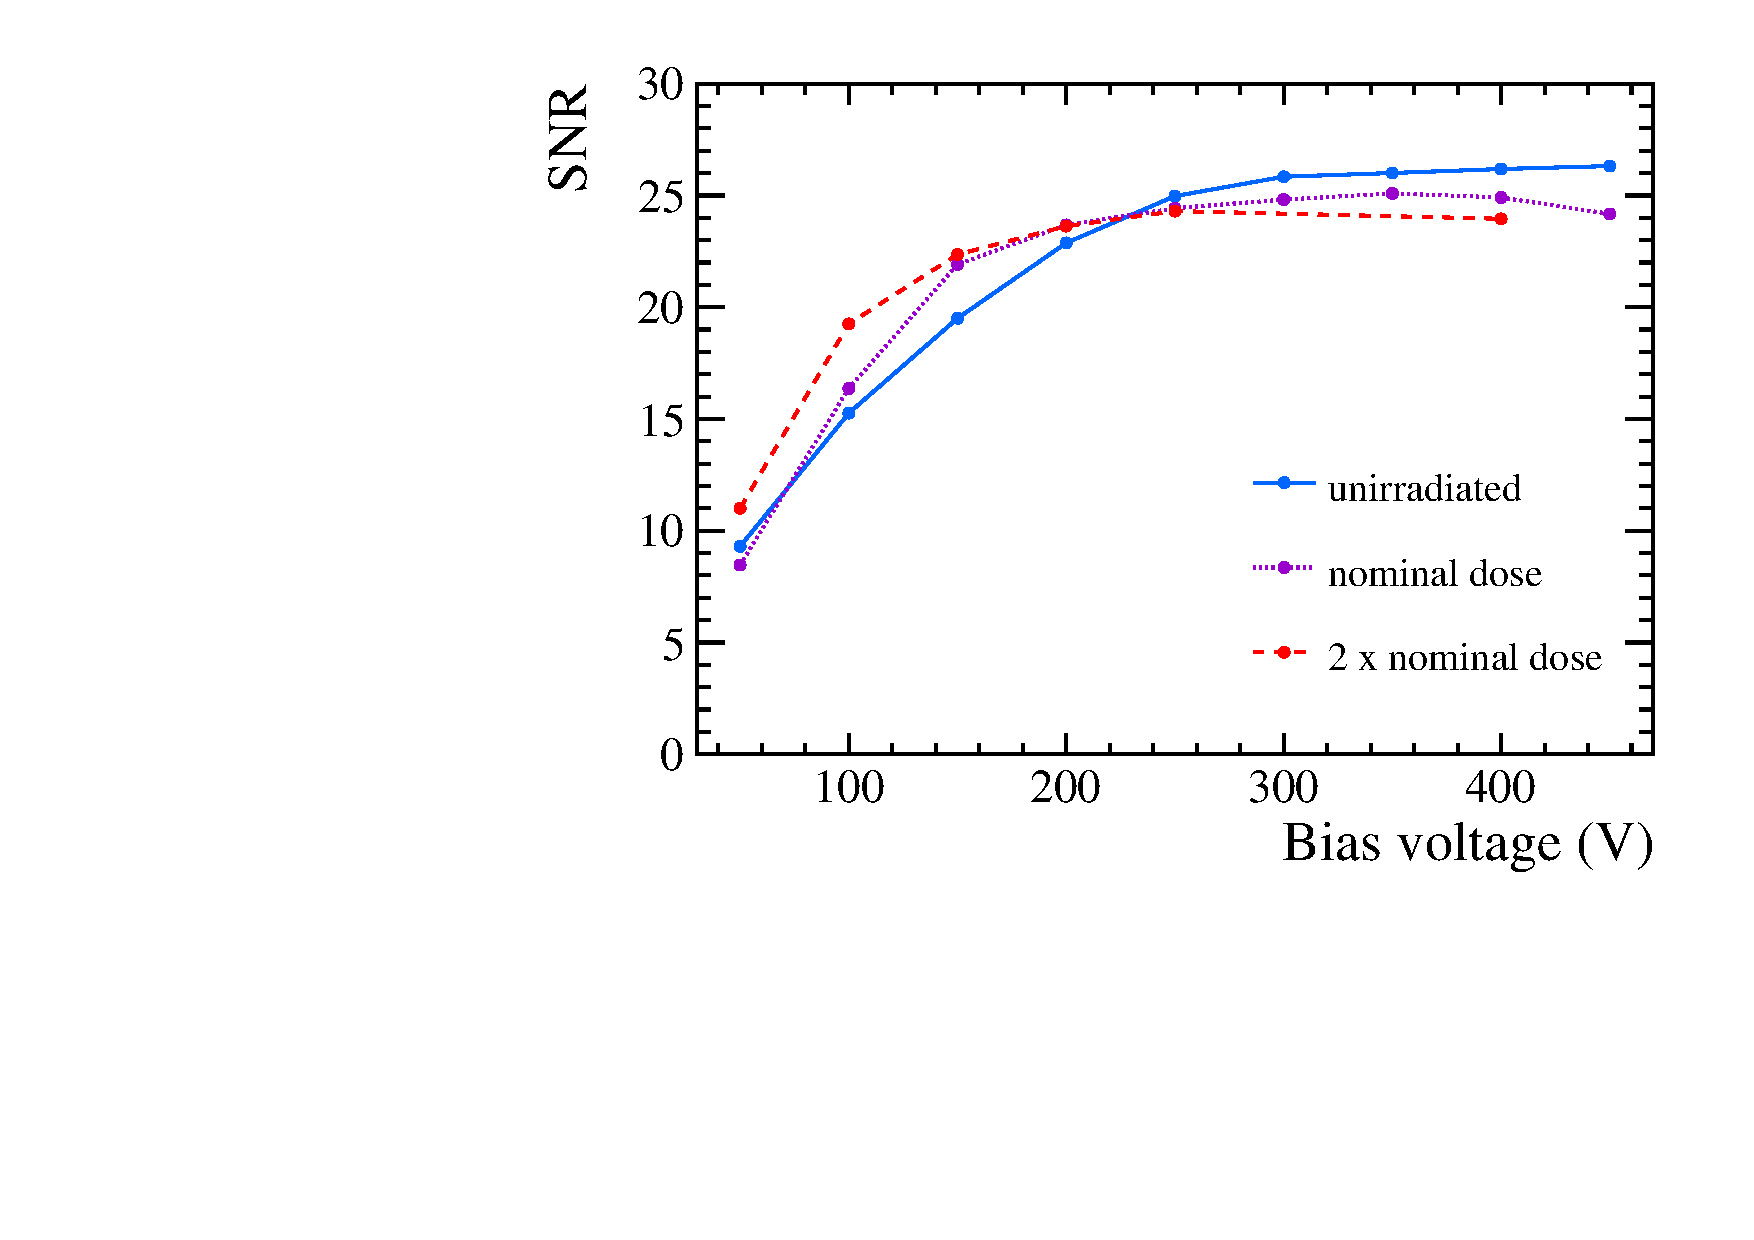
\includegraphics[width=0.47\textwidth]{figs/CombineSNRvsBias/cSNRvsBias_FanIn_Top.pdf}
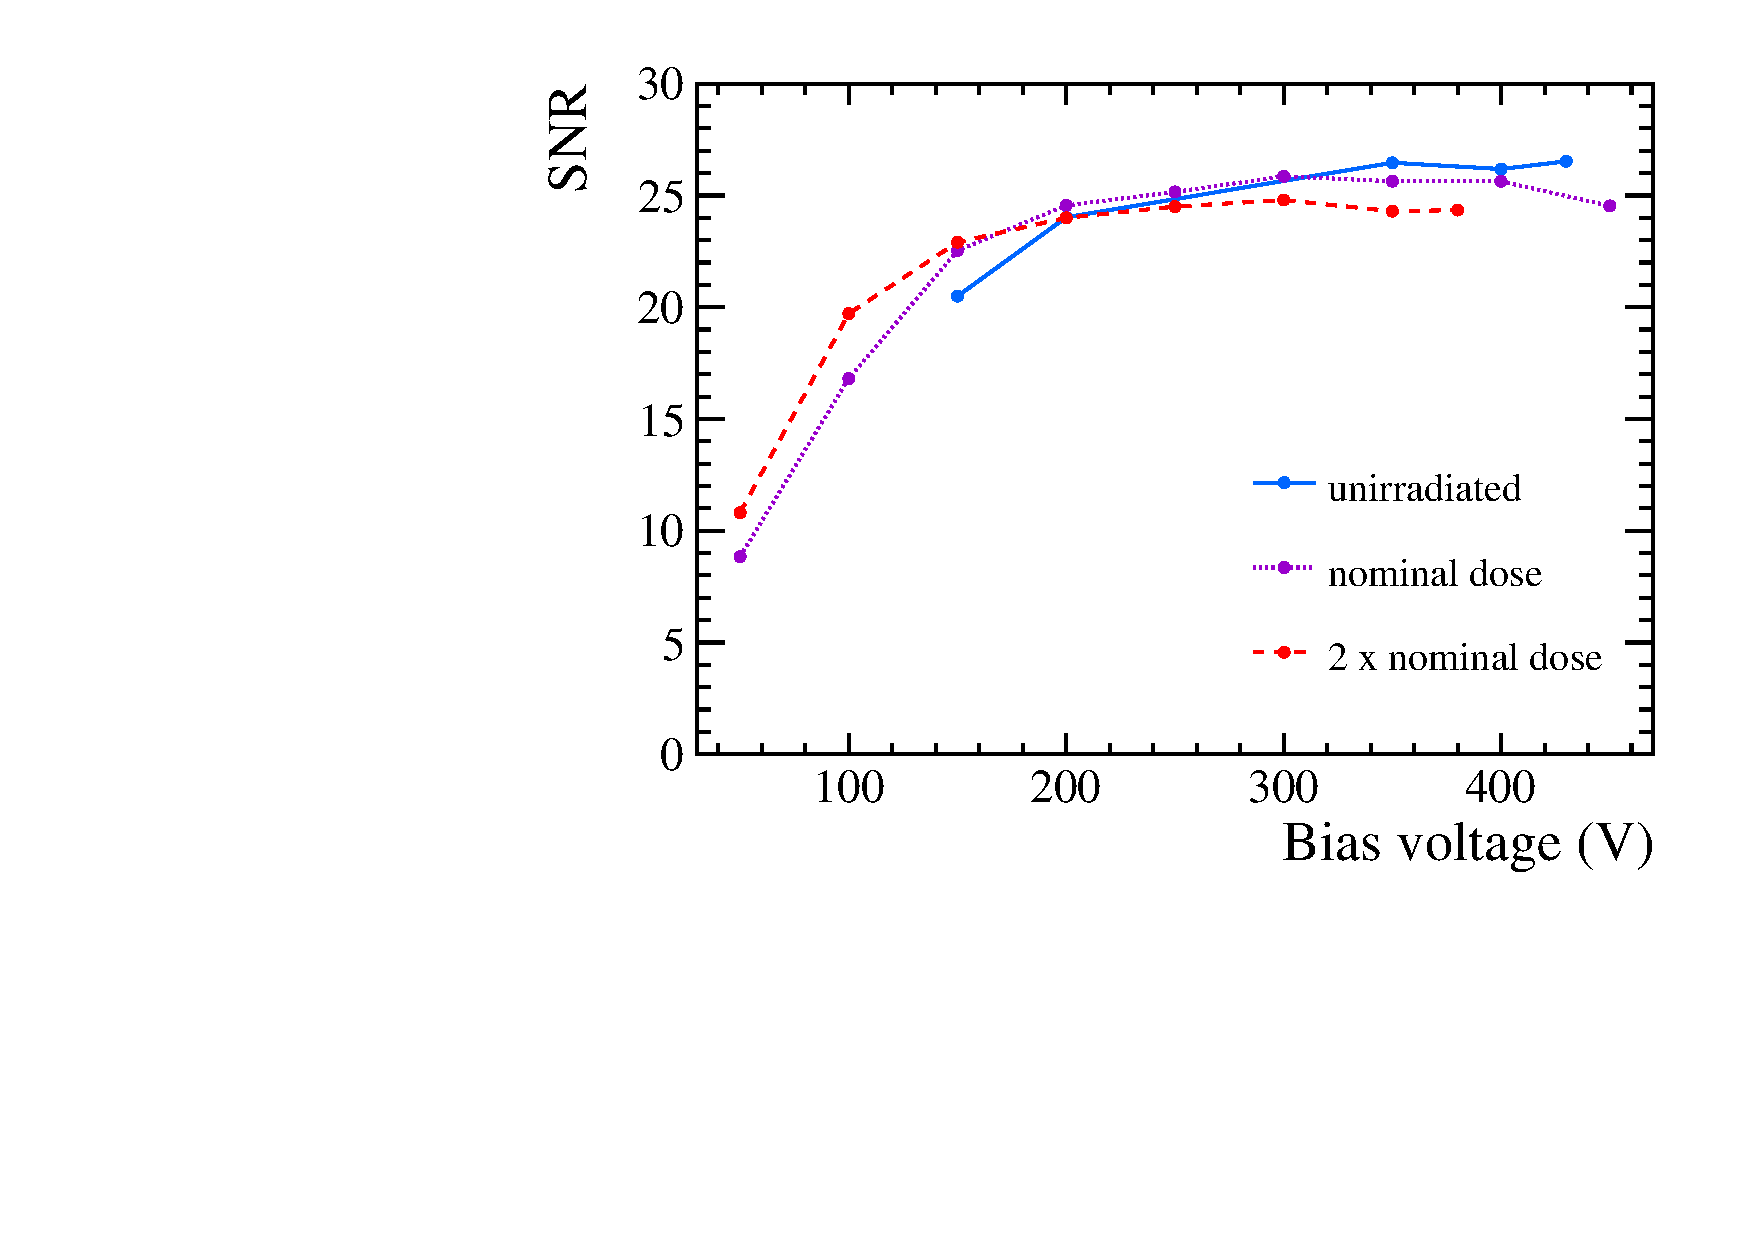
\includegraphics[width=0.47\textwidth]{figs/CombineSNRvsBias/cSNRvsBias_FanUp_Back.pdf}
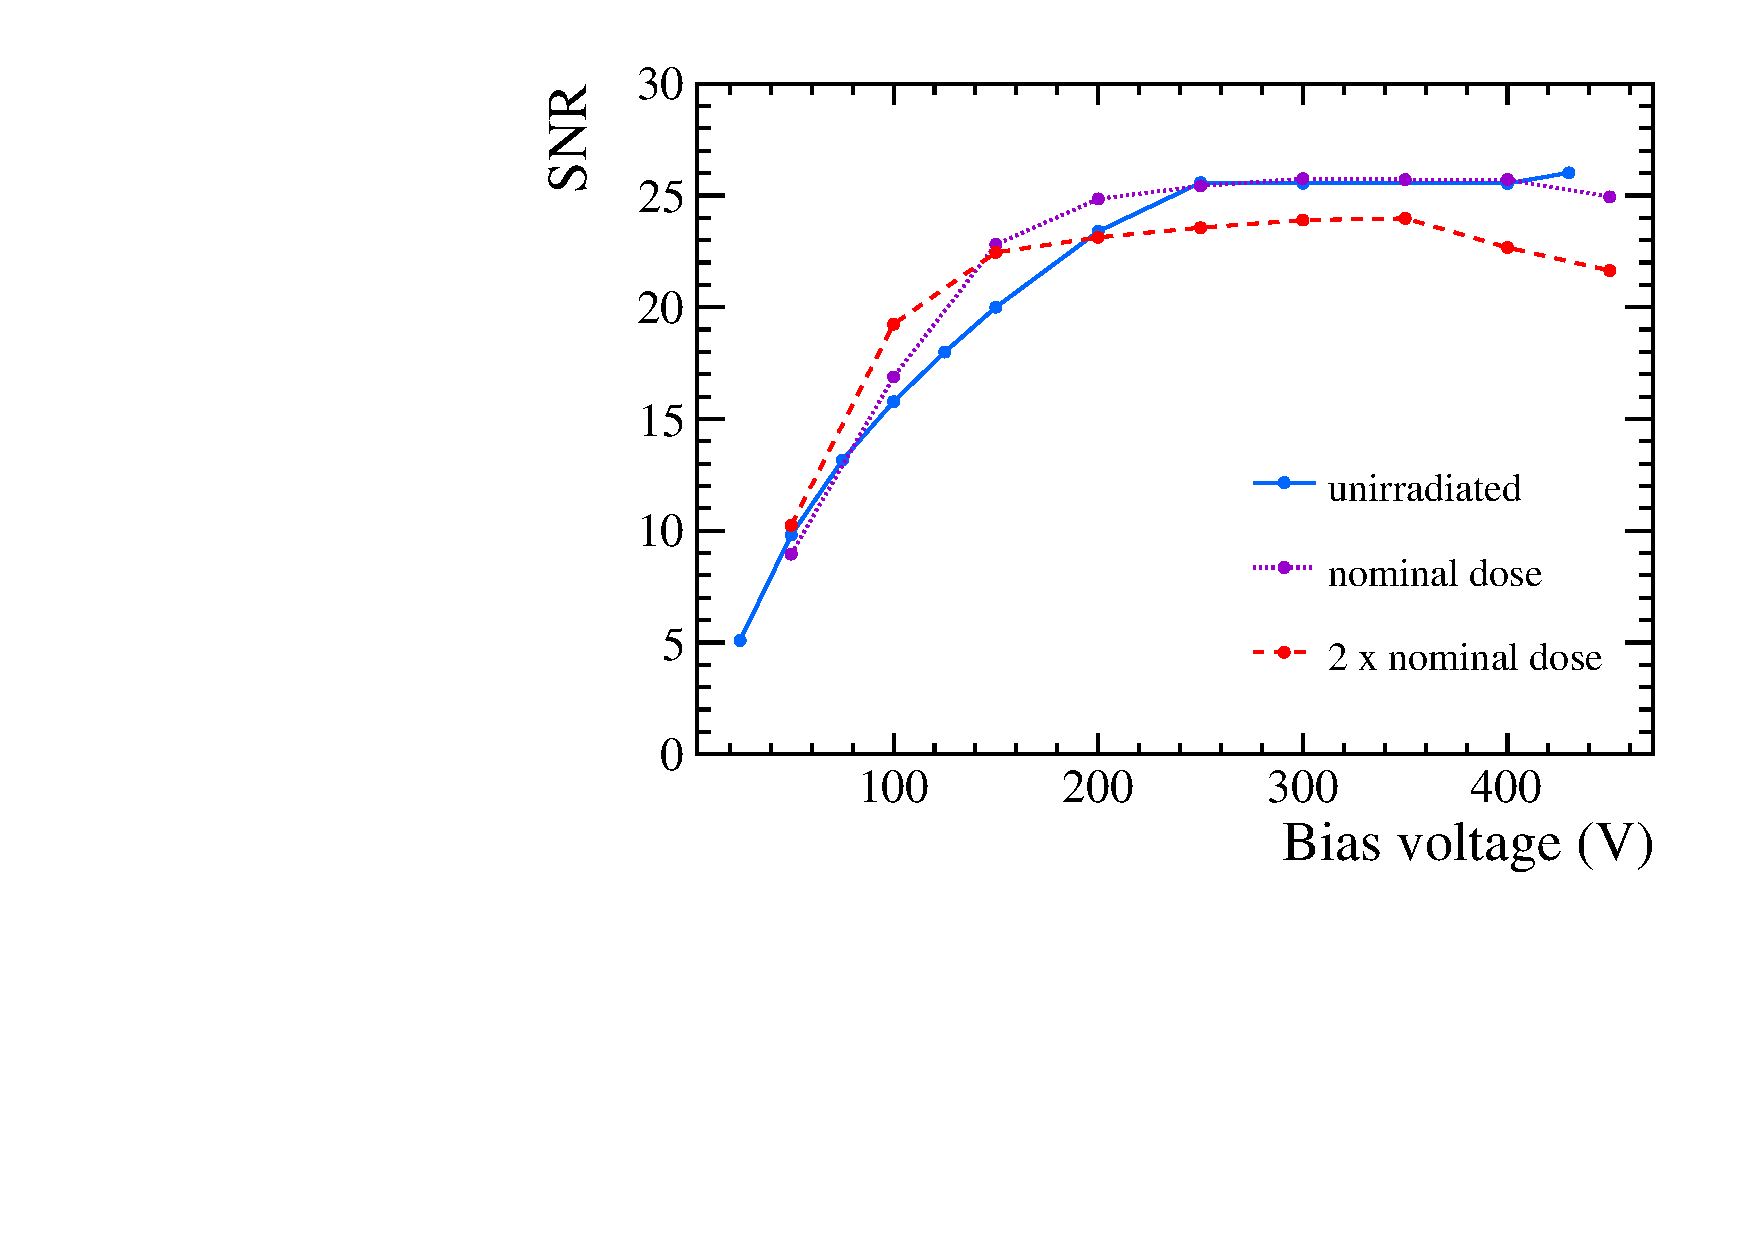
\includegraphics[width=0.47\textwidth]{figs/CombineSNRvsBias/cSNRvsBias_FanUp_Top.pdf}
\caption[SNR as a function of the applied bias voltage for the mini sensors.]{SNR as a function of the applied bias voltage for the mini sensors with the fan-in (top) and fan-up (bottom) pitch adapter and the back side (left) and top side (right) biasing scheme. The three curves refer to different radiation doses: no irradiation (solid blue line), nominal dose (dotted violet line), and twice the nominal dose (dashed red line).}
\label{fig:DepletionVoltageM}
\end{figure}

\begin{figure}[]
\centering
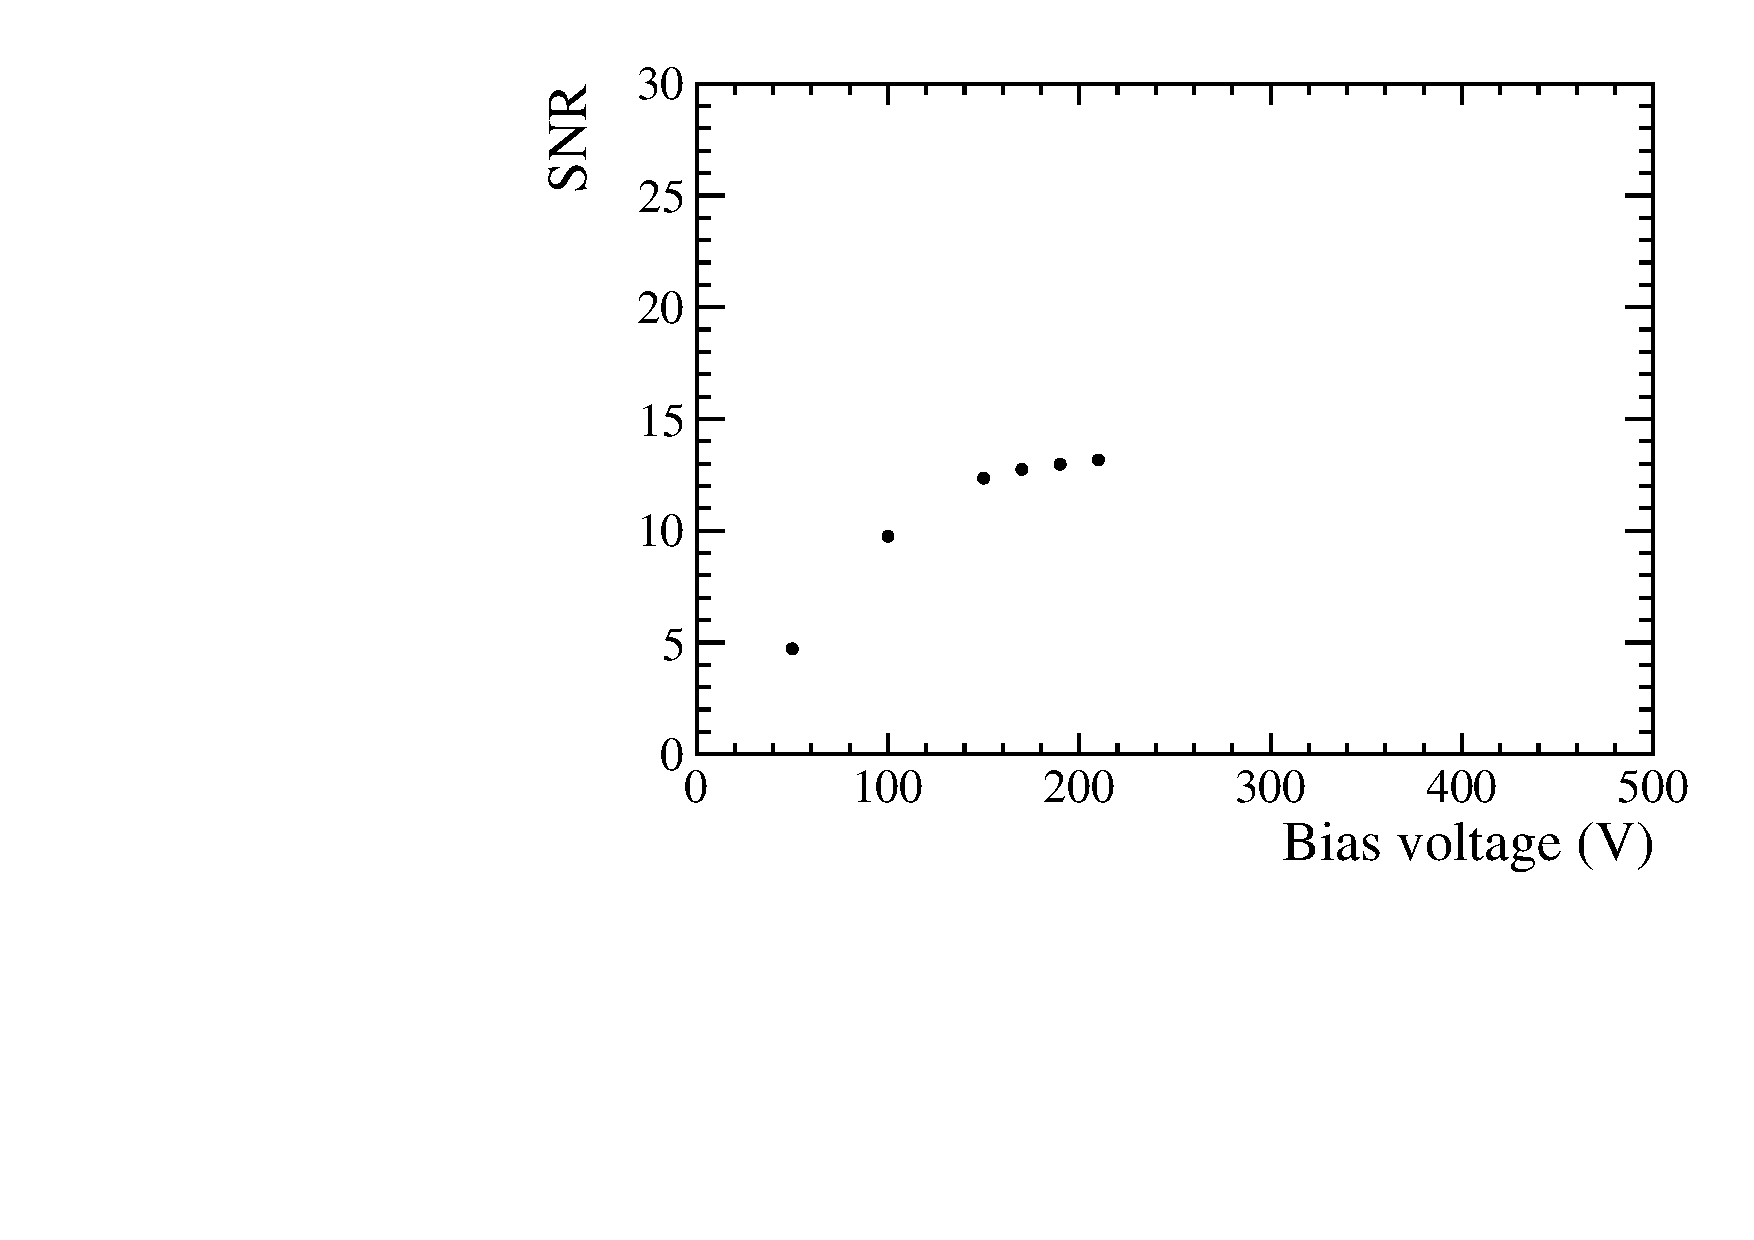
\includegraphics[width=0.47\textwidth]{figs/SNRvsBias/cSNRvsBias_F1_FanUp_Back.pdf}
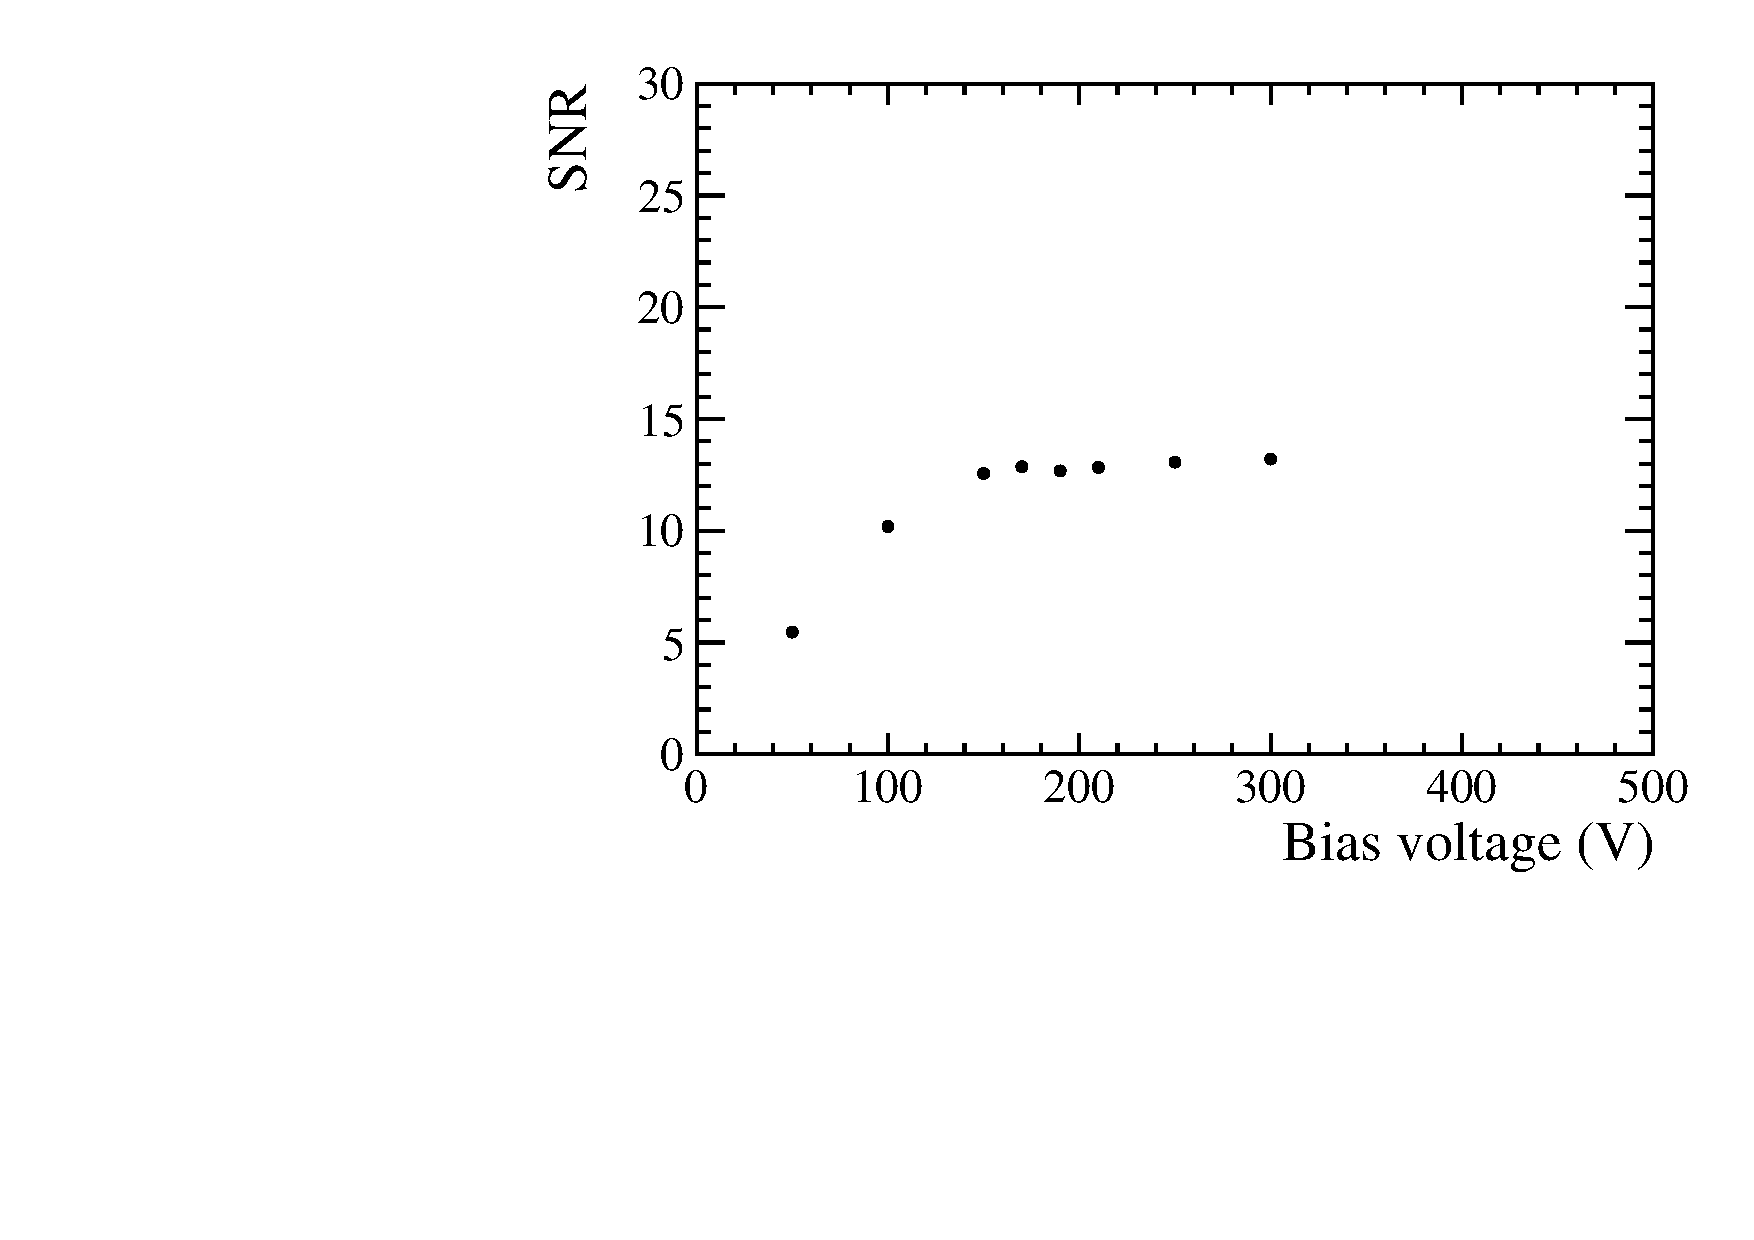
\includegraphics[width=0.47\textwidth]{figs/SNRvsBias/cSNRvsBias_F1_FanUp_Top.pdf}
\caption[SNR as a function of the applied bias voltage for the half size sensor.]{SNR as a function of the applied bias voltage for the half size sensor with the back side (left) and top side (right) biasing scheme.}
\label{fig:DepletionVoltageF}
\end{figure}

For the mini sensors, the depletion voltage decreases with increasing radiation doses for both pitch adapters and for both biasing schemes. This might be due to an increase in the noise (to be checked).

\begin{figure}[]
\centering
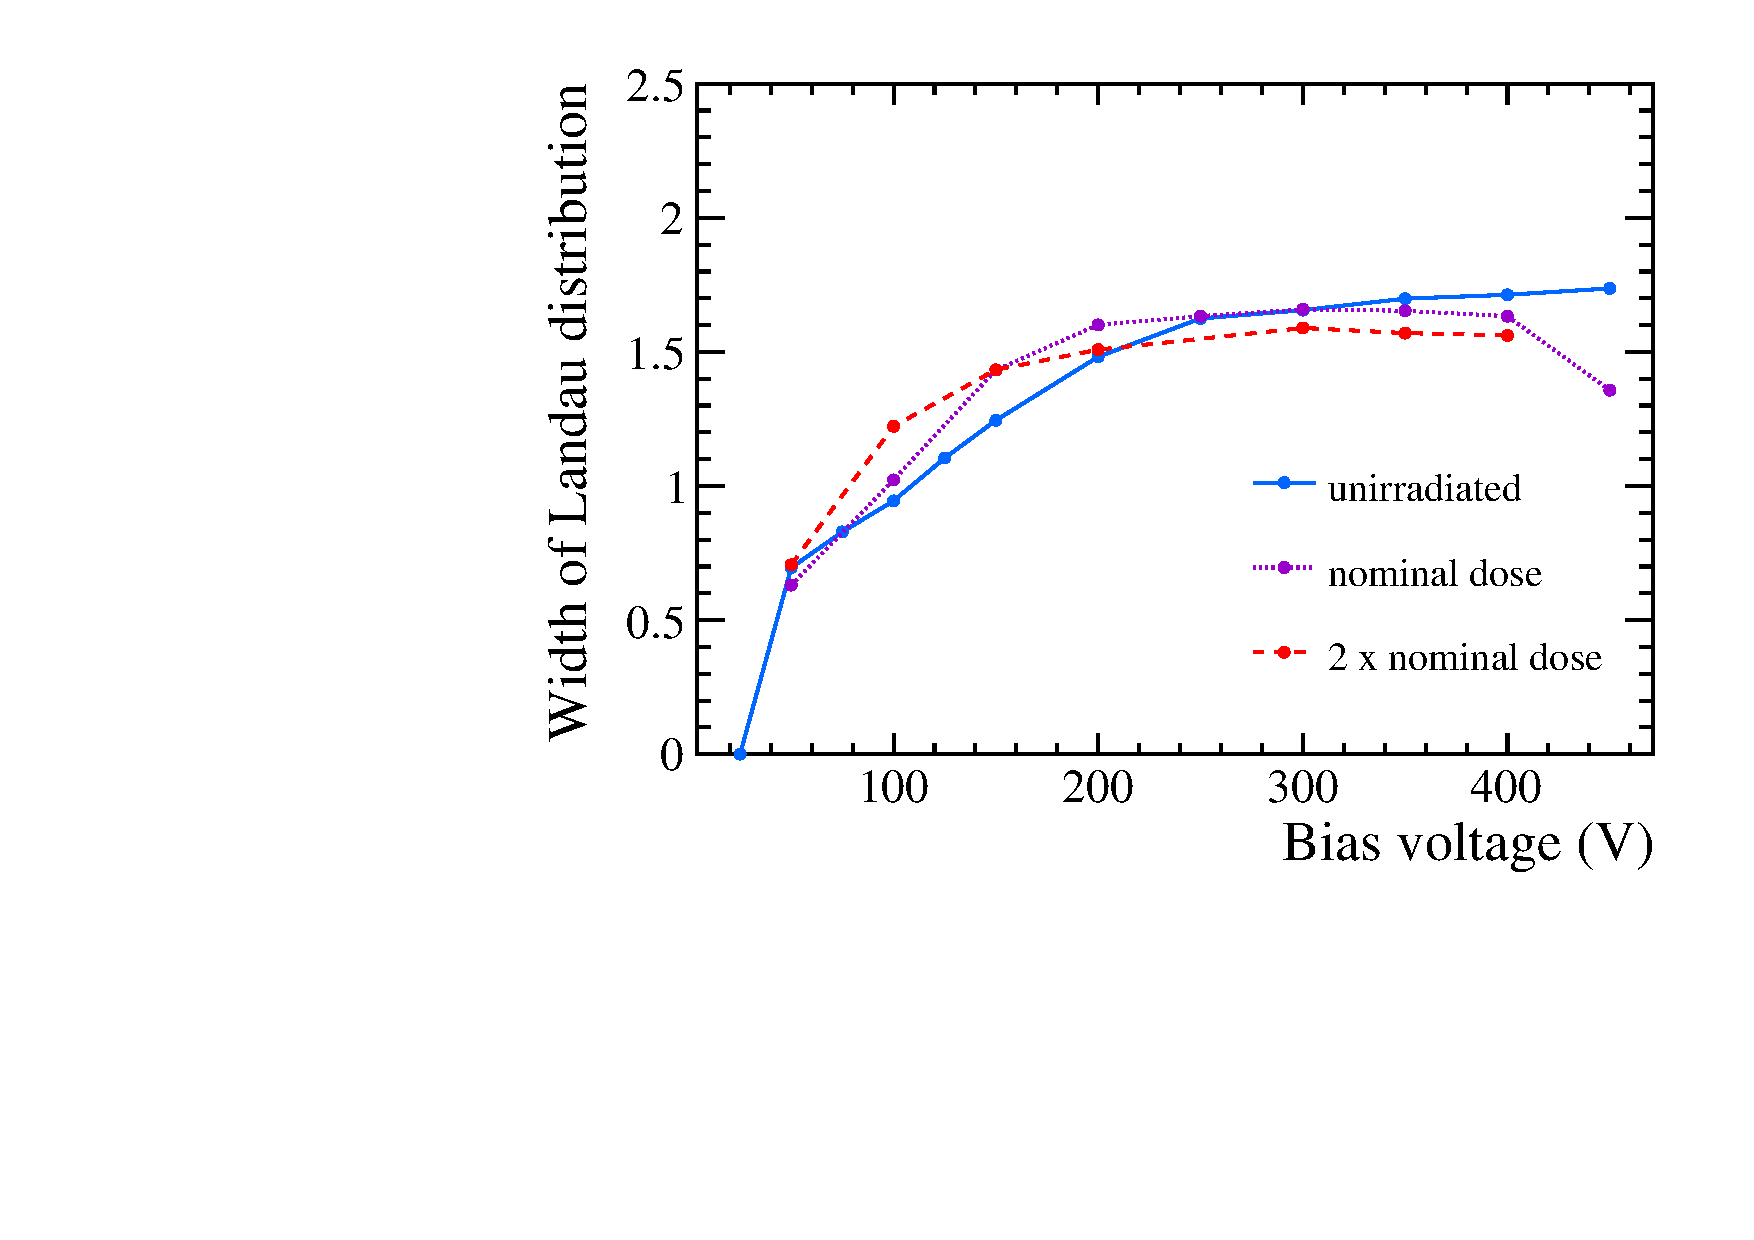
\includegraphics[width=0.47\textwidth]{figs/CombineSNRvsBias/cwidthvsBias_FanIn_Back.pdf}
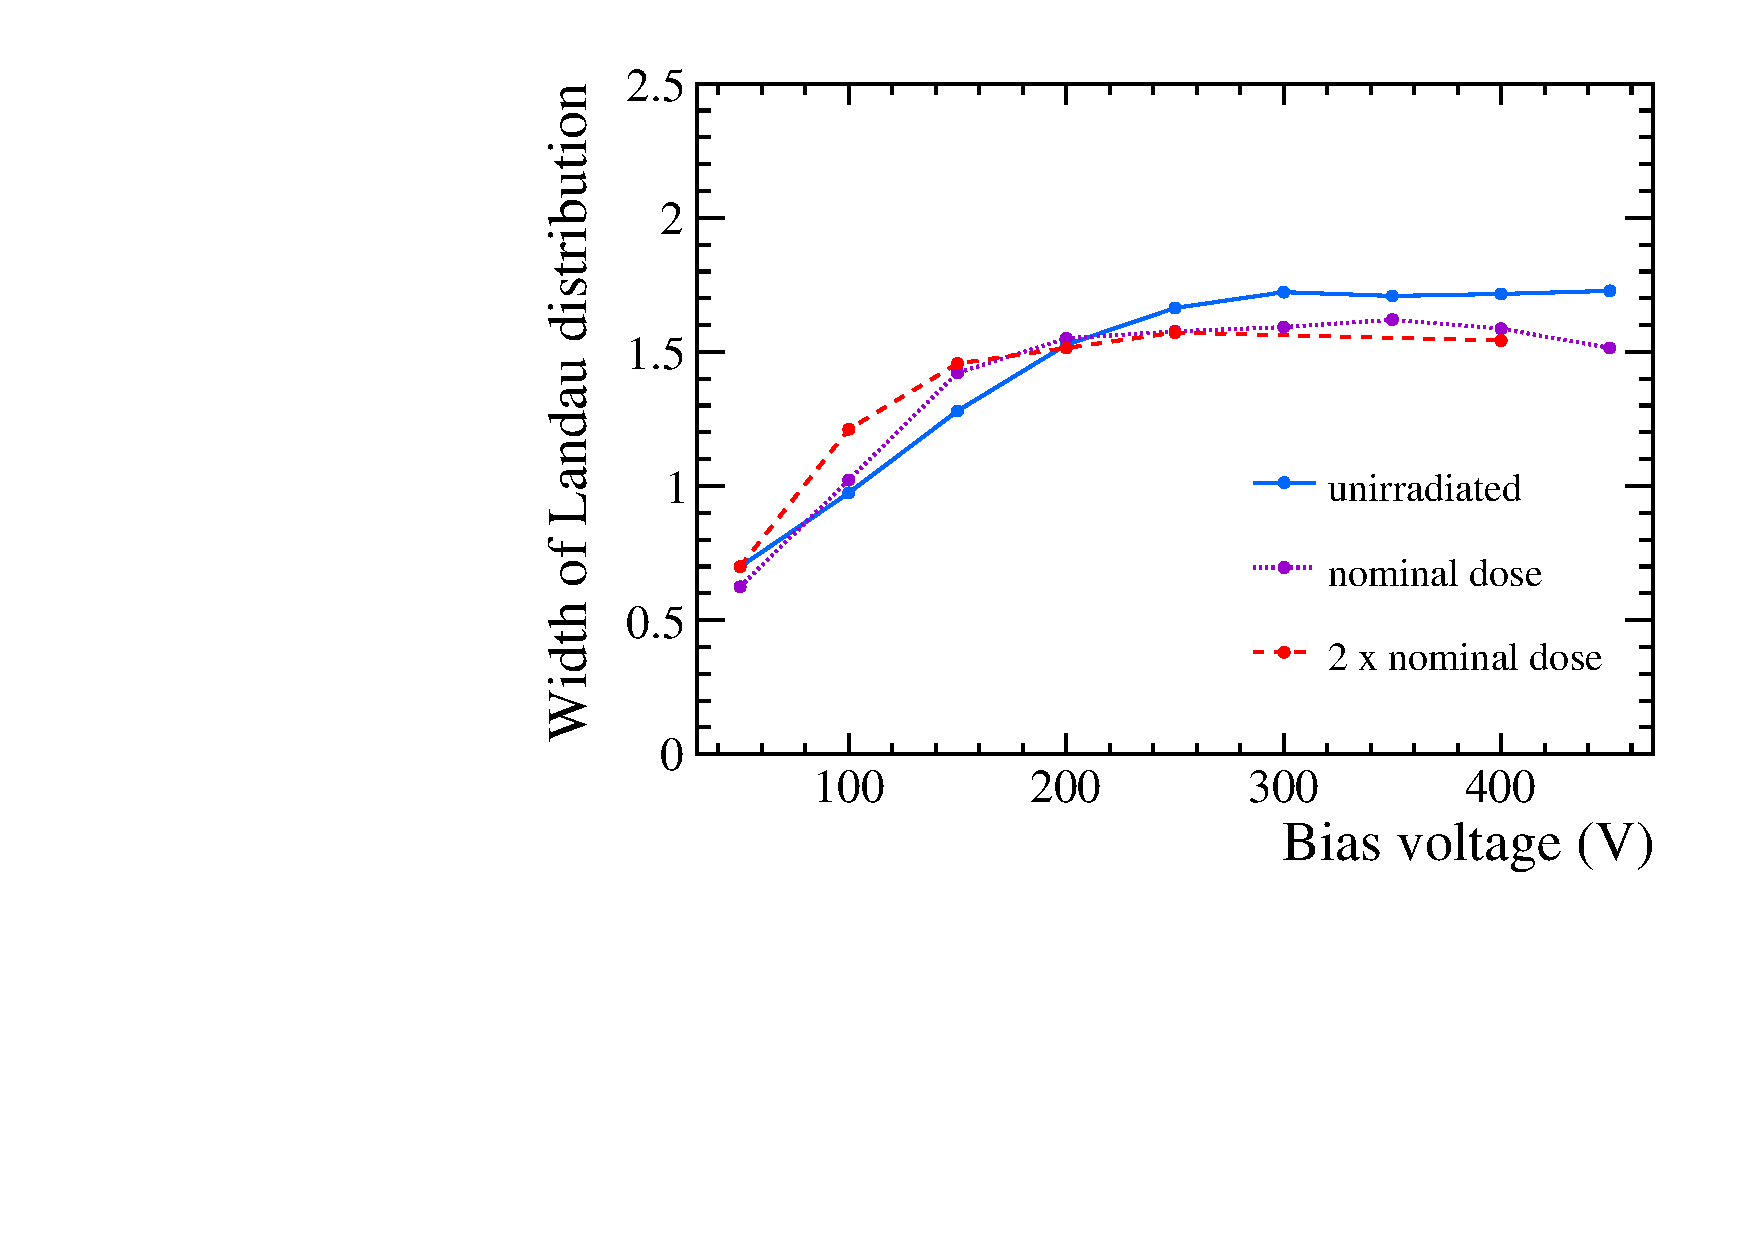
\includegraphics[width=0.47\textwidth]{figs/CombineSNRvsBias/cwidthvsBias_FanIn_Top.pdf}
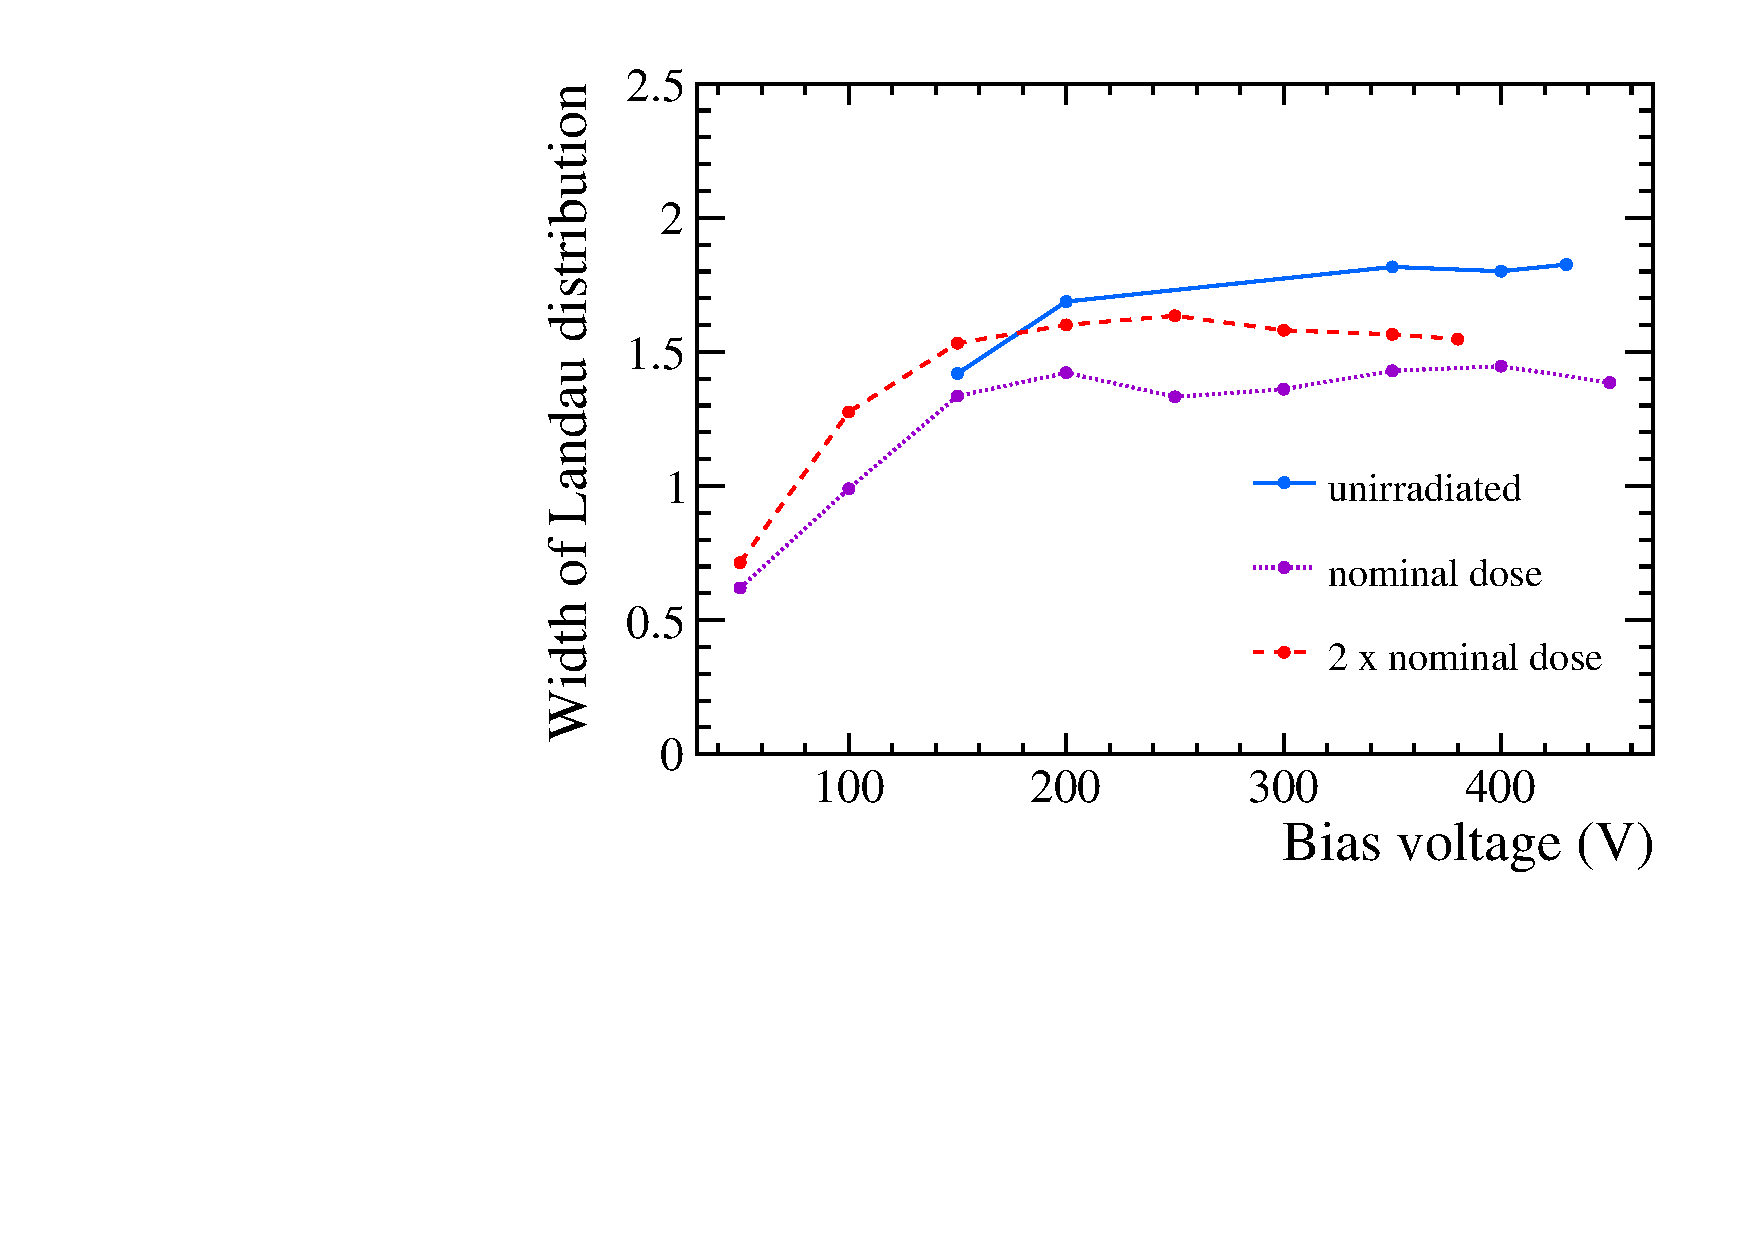
\includegraphics[width=0.47\textwidth]{figs/CombineSNRvsBias/cwidthvsBias_FanUp_Back.pdf}
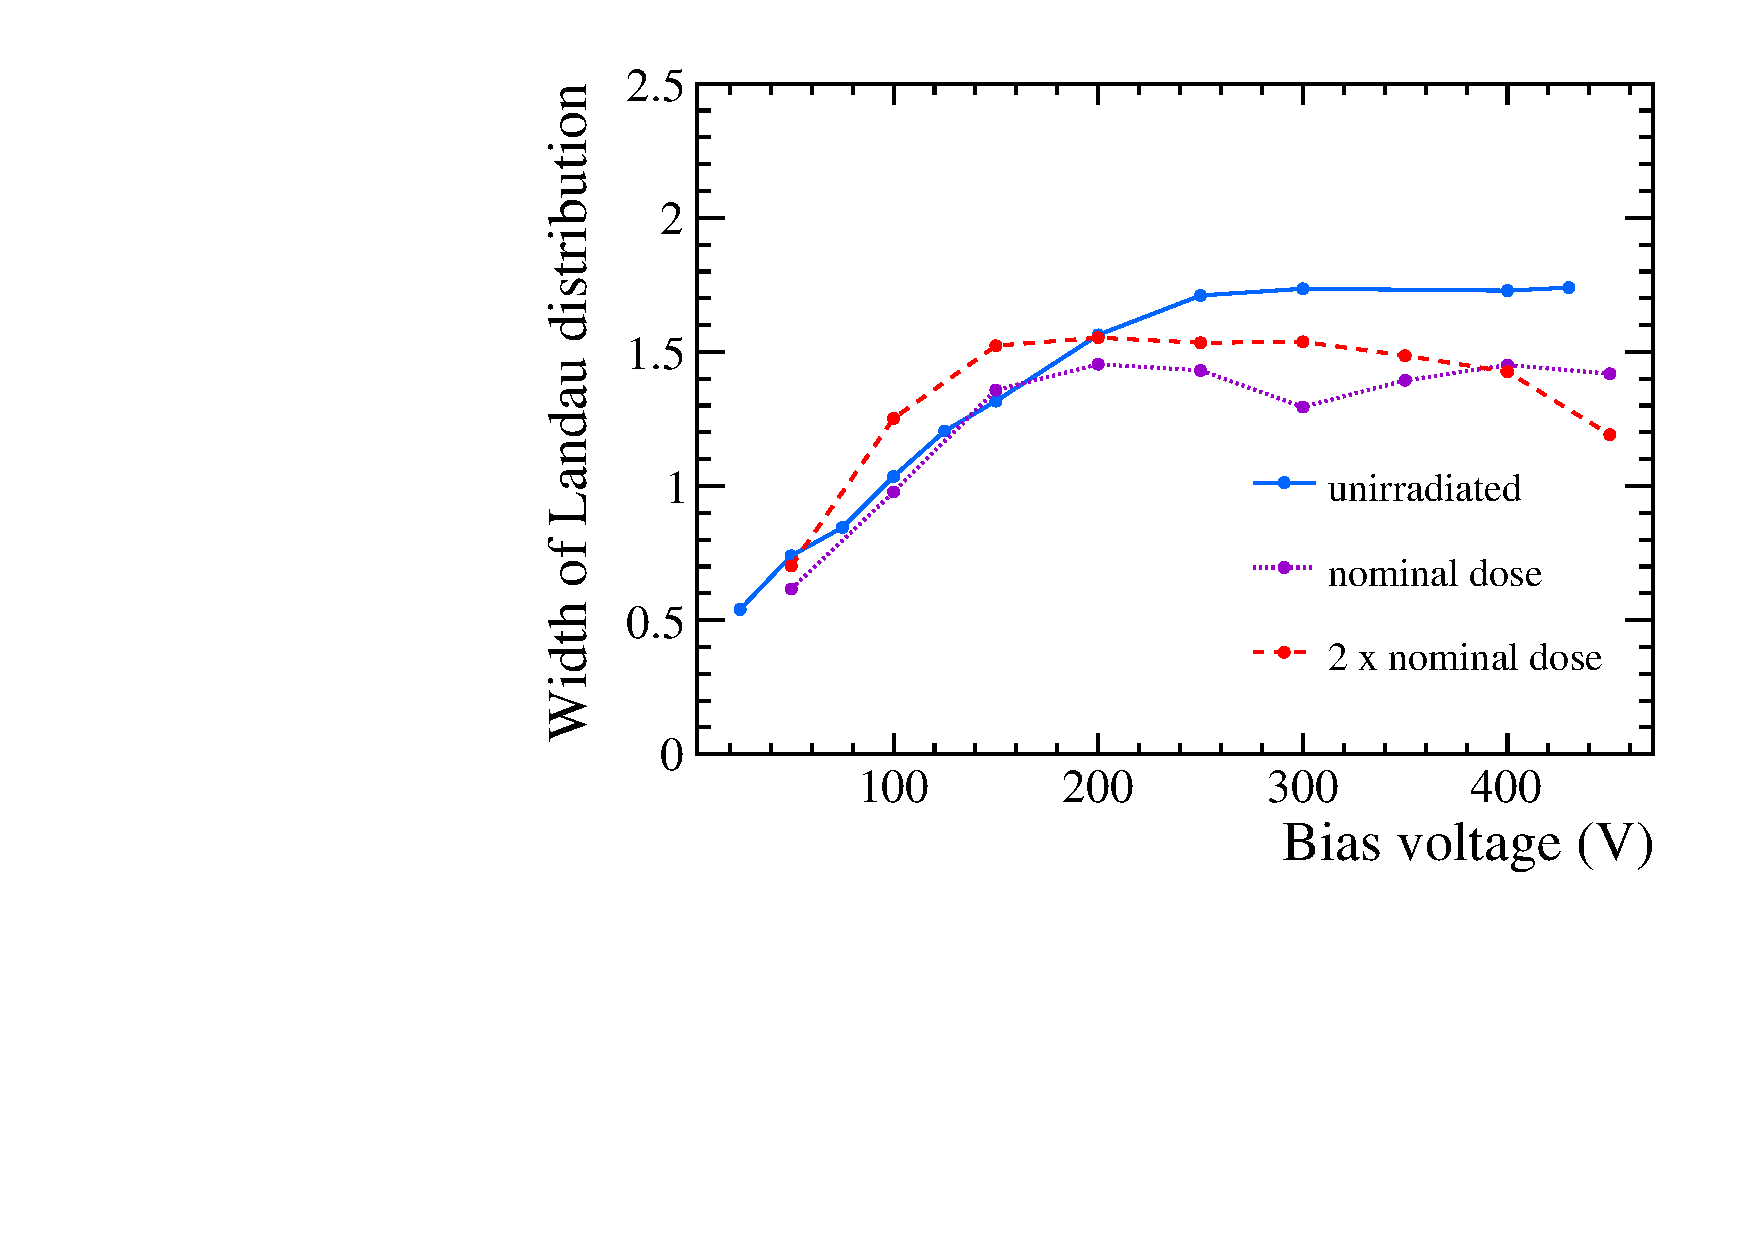
\includegraphics[width=0.47\textwidth]{figs/CombineSNRvsBias/cwidthvsBias_FanUp_Top.pdf}
\caption[Parameter $\sigma$ as a function of the applied bias voltage for the mini sensors.]{Parameter $\sigma$  as a function of the applied bias voltage for the mini sensors with the fan-in (top) and fan-up (bottom) pitch adapter and the back side (left) and top side (right) biasing scheme.}
\label{fig:DepletionVoltage2M}
\end{figure}

\begin{figure}[]
\centering
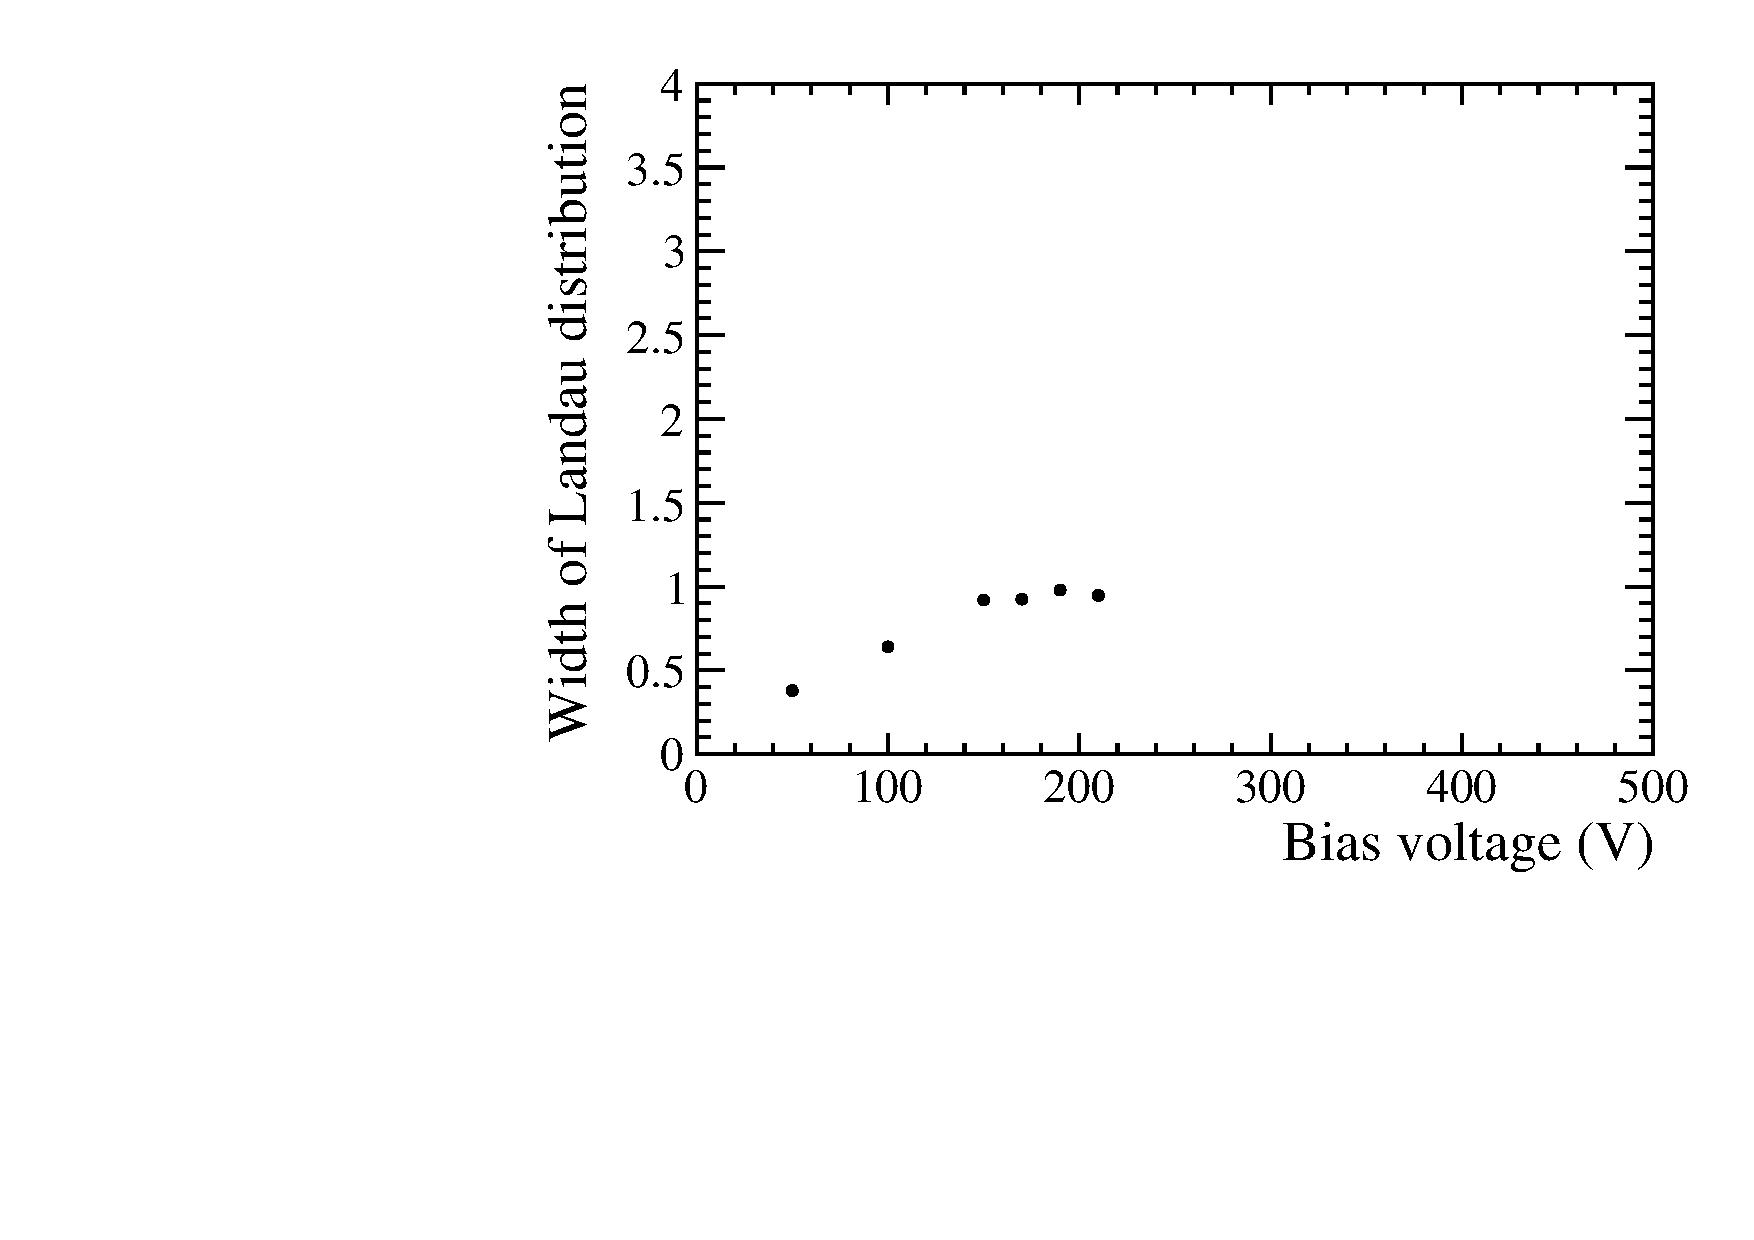
\includegraphics[width=0.47\textwidth]{figs/SNRvsBias/cwidthvsBias_F1_FanUp_Back.pdf}
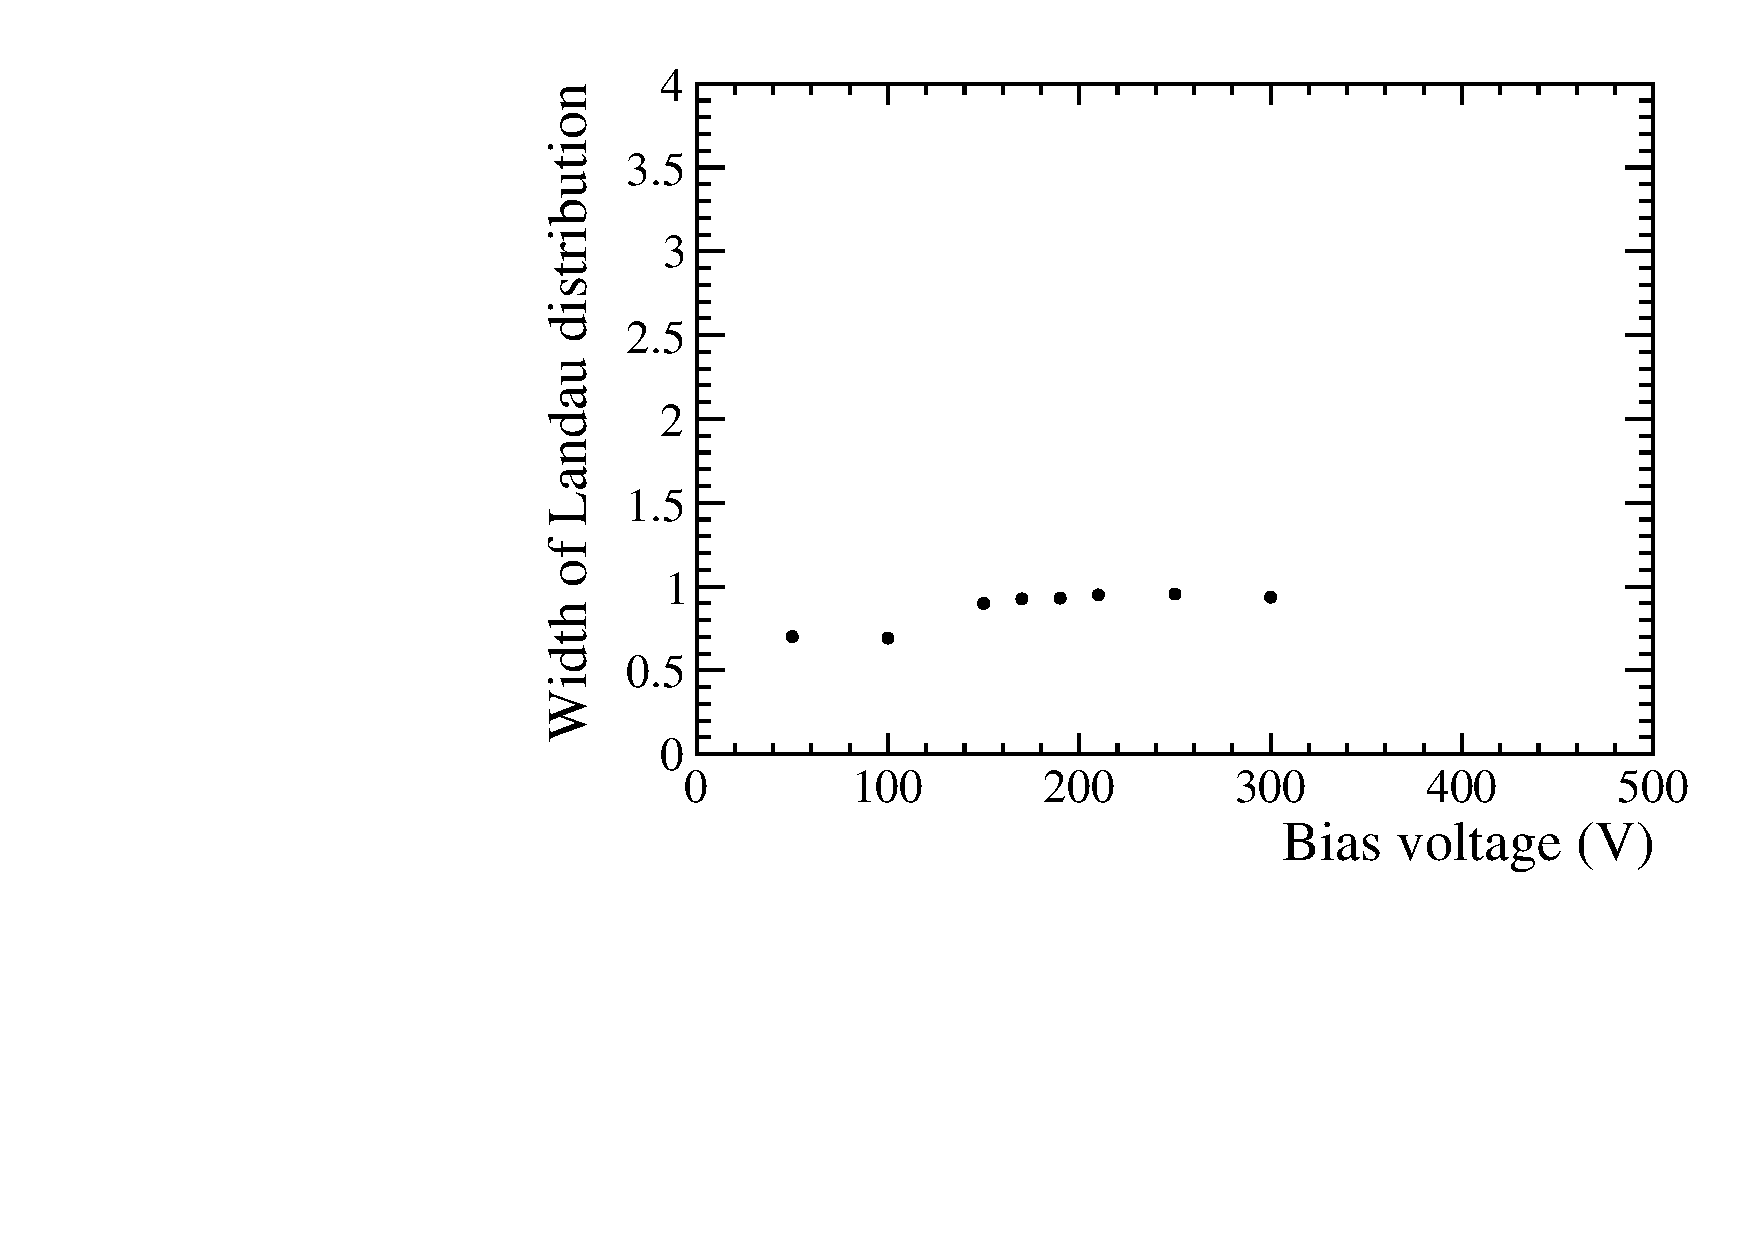
\includegraphics[width=0.47\textwidth]{figs/SNRvsBias/cwidthvsBias_F1_FanUp_Top.pdf}
\caption[Parameter $\sigma$ as a function of the applied bias voltage for the half size sensor.]{Parameter $\sigma$ as a function of the applied bias voltage for the half size sensor with the back side (left) and top side (right) biasing scheme.}
\label{fig:DepletionVoltage2F}
\end{figure}